% Filename: history_timeline1@latex_with_vim.tex
% This code is part of LaTeX with Vim.
% 
% Description: TikZ for teachers is free book about TikZ and Sage.
% 
% Created: 30.03.12 07:55:25 PM
% Last Change: 30.03.12 07:56:41 PM
% 
% Author: Raniere Gaia Costa da Silva, r.gaia.cs@gmail.com
% Organization:  
% 
% Copyright (c) 2010, 2011, 2012, Raniere Gaia Costa da Silva. All rights 
% reserved.
% 
% This file is license under the terms of a Creative Commons Attribution 
% 3.0 Unported License, or (at your option) any later version. More details
% at <http://creativecommons.org/licenses/by/3.0/>.
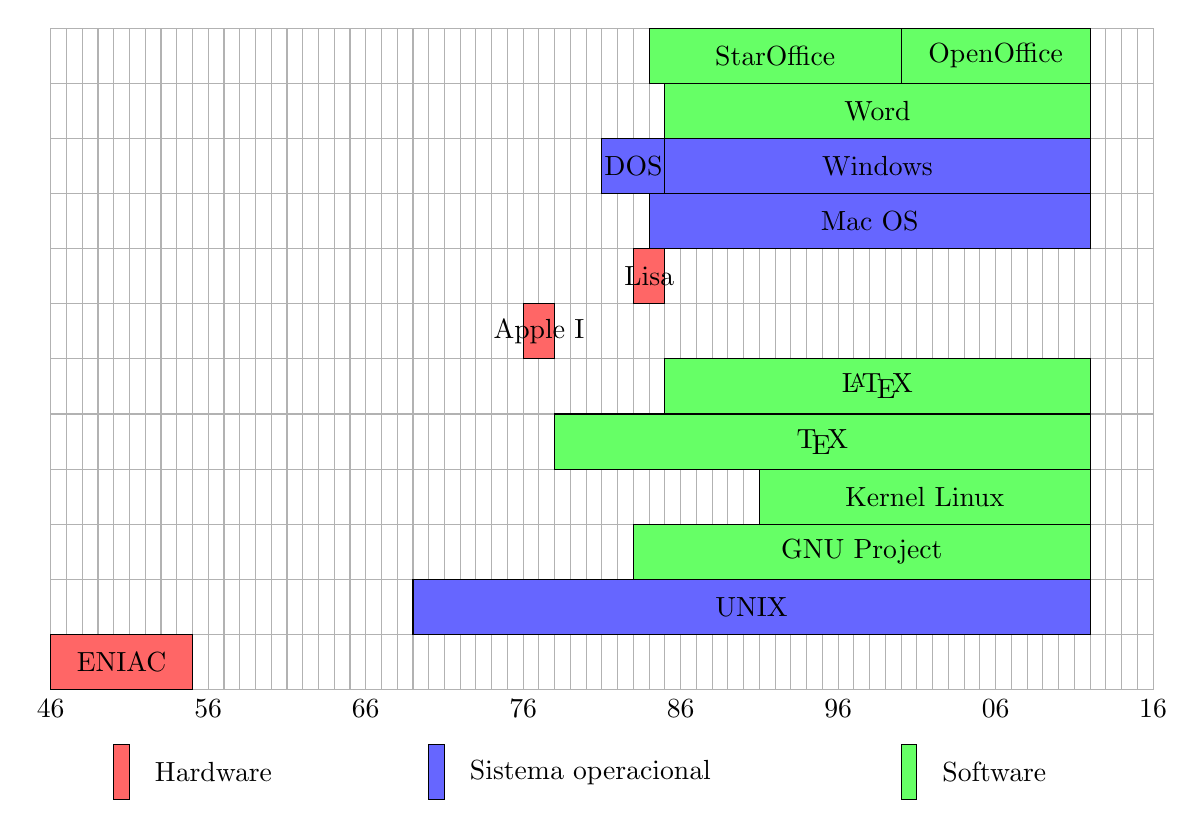
\begin{tikzpicture}[xscale=0.2, yscale=0.7]
    \draw[gray!60] (46,0) grid (116,12);
    \foreach \y in {46, 56, ..., 96}{
        \node[below] at (\y, 0) {\y};
    }
    \node[below] at (106,0) {06};
    \node[below] at (116,0) {16};

    \draw[fill=red!60] (50,-1) rectangle ++(1,-1) ++(1,.5) node[right]{Hardware};
    \draw[fill=blue!60] (70,-1) rectangle ++(1,-1) ++(1,.5) node[right]{Sistema operacional};
    \draw[fill=green!60] (100,-1) rectangle ++(1,-1) ++(1,.5) node[right]{Software};

    \draw[fill=red!60] (46,0) rectangle (55,1) node[midway]{ENIAC};
    \draw[fill=blue!60] (69,1) rectangle (112,2) node[midway]{UNIX};
    \draw[fill=green!60] (83,2) rectangle (112,3) node[midway]{GNU Project};
    \draw[fill=green!60] (91,3) rectangle (112,4) node[midway]{Kernel Linux};
    \draw[fill=green!60] (78,4) rectangle (112,5) node[midway]{\TeX};
    \draw[fill=green!60] (85,5) rectangle (112,6) node[midway]{\LaTeX};
    \draw[fill=red!60] (76,6) rectangle (78,7) node[midway]{Apple I};
    \draw[fill=red!60] (83,7) rectangle (85,8) node[midway]{Lisa};
    \draw[fill=blue!60] (84,8) rectangle (112,9) node[midway]{Mac OS};
    \draw[fill=blue!60] (81,9) rectangle (85,10) node[midway]{DOS};
    \draw[fill=blue!60] (85,9) rectangle (112,10) node[midway]{Windows};
    \draw[fill=green!60] (85,10) rectangle (112,11) node[midway]{Word};
    \draw[fill=green!60] (84,11) rectangle (100,12) node[midway]{StarOffice};
    \draw[fill=green!60] (100,11) rectangle (112,12) node[midway]{OpenOffice};
\end{tikzpicture}
